\documentclass[]{article}
\usepackage{lmodern}
\usepackage{amssymb,amsmath}
\usepackage{ifxetex,ifluatex}
\usepackage{fixltx2e} % provides \textsubscript
\ifnum 0\ifxetex 1\fi\ifluatex 1\fi=0 % if pdftex
  \usepackage[T1]{fontenc}
  \usepackage[utf8]{inputenc}
\else % if luatex or xelatex
  \ifxetex
    \usepackage{mathspec}
  \else
    \usepackage{fontspec}
  \fi
  \defaultfontfeatures{Ligatures=TeX,Scale=MatchLowercase}
\fi
% use upquote if available, for straight quotes in verbatim environments
\IfFileExists{upquote.sty}{\usepackage{upquote}}{}
% use microtype if available
\IfFileExists{microtype.sty}{%
\usepackage{microtype}
\UseMicrotypeSet[protrusion]{basicmath} % disable protrusion for tt fonts
}{}
\usepackage[margin=1in]{geometry}
\usepackage{hyperref}
\hypersetup{unicode=true,
            pdftitle={DRAFT: Analysis of the reporting styles using generalized ordered threshold models.},
            pdfauthor={Maciej J. Dańko},
            pdfborder={0 0 0},
            breaklinks=true}
\urlstyle{same}  % don't use monospace font for urls
\usepackage{color}
\usepackage{fancyvrb}
\newcommand{\VerbBar}{|}
\newcommand{\VERB}{\Verb[commandchars=\\\{\}]}
\DefineVerbatimEnvironment{Highlighting}{Verbatim}{commandchars=\\\{\}}
% Add ',fontsize=\small' for more characters per line
\usepackage{framed}
\definecolor{shadecolor}{RGB}{248,248,248}
\newenvironment{Shaded}{\begin{snugshade}}{\end{snugshade}}
\newcommand{\AlertTok}[1]{\textcolor[rgb]{0.94,0.16,0.16}{#1}}
\newcommand{\AnnotationTok}[1]{\textcolor[rgb]{0.56,0.35,0.01}{\textbf{\textit{#1}}}}
\newcommand{\AttributeTok}[1]{\textcolor[rgb]{0.77,0.63,0.00}{#1}}
\newcommand{\BaseNTok}[1]{\textcolor[rgb]{0.00,0.00,0.81}{#1}}
\newcommand{\BuiltInTok}[1]{#1}
\newcommand{\CharTok}[1]{\textcolor[rgb]{0.31,0.60,0.02}{#1}}
\newcommand{\CommentTok}[1]{\textcolor[rgb]{0.56,0.35,0.01}{\textit{#1}}}
\newcommand{\CommentVarTok}[1]{\textcolor[rgb]{0.56,0.35,0.01}{\textbf{\textit{#1}}}}
\newcommand{\ConstantTok}[1]{\textcolor[rgb]{0.00,0.00,0.00}{#1}}
\newcommand{\ControlFlowTok}[1]{\textcolor[rgb]{0.13,0.29,0.53}{\textbf{#1}}}
\newcommand{\DataTypeTok}[1]{\textcolor[rgb]{0.13,0.29,0.53}{#1}}
\newcommand{\DecValTok}[1]{\textcolor[rgb]{0.00,0.00,0.81}{#1}}
\newcommand{\DocumentationTok}[1]{\textcolor[rgb]{0.56,0.35,0.01}{\textbf{\textit{#1}}}}
\newcommand{\ErrorTok}[1]{\textcolor[rgb]{0.64,0.00,0.00}{\textbf{#1}}}
\newcommand{\ExtensionTok}[1]{#1}
\newcommand{\FloatTok}[1]{\textcolor[rgb]{0.00,0.00,0.81}{#1}}
\newcommand{\FunctionTok}[1]{\textcolor[rgb]{0.00,0.00,0.00}{#1}}
\newcommand{\ImportTok}[1]{#1}
\newcommand{\InformationTok}[1]{\textcolor[rgb]{0.56,0.35,0.01}{\textbf{\textit{#1}}}}
\newcommand{\KeywordTok}[1]{\textcolor[rgb]{0.13,0.29,0.53}{\textbf{#1}}}
\newcommand{\NormalTok}[1]{#1}
\newcommand{\OperatorTok}[1]{\textcolor[rgb]{0.81,0.36,0.00}{\textbf{#1}}}
\newcommand{\OtherTok}[1]{\textcolor[rgb]{0.56,0.35,0.01}{#1}}
\newcommand{\PreprocessorTok}[1]{\textcolor[rgb]{0.56,0.35,0.01}{\textit{#1}}}
\newcommand{\RegionMarkerTok}[1]{#1}
\newcommand{\SpecialCharTok}[1]{\textcolor[rgb]{0.00,0.00,0.00}{#1}}
\newcommand{\SpecialStringTok}[1]{\textcolor[rgb]{0.31,0.60,0.02}{#1}}
\newcommand{\StringTok}[1]{\textcolor[rgb]{0.31,0.60,0.02}{#1}}
\newcommand{\VariableTok}[1]{\textcolor[rgb]{0.00,0.00,0.00}{#1}}
\newcommand{\VerbatimStringTok}[1]{\textcolor[rgb]{0.31,0.60,0.02}{#1}}
\newcommand{\WarningTok}[1]{\textcolor[rgb]{0.56,0.35,0.01}{\textbf{\textit{#1}}}}
\usepackage{graphicx,grffile}
\makeatletter
\def\maxwidth{\ifdim\Gin@nat@width>\linewidth\linewidth\else\Gin@nat@width\fi}
\def\maxheight{\ifdim\Gin@nat@height>\textheight\textheight\else\Gin@nat@height\fi}
\makeatother
% Scale images if necessary, so that they will not overflow the page
% margins by default, and it is still possible to overwrite the defaults
% using explicit options in \includegraphics[width, height, ...]{}
\setkeys{Gin}{width=\maxwidth,height=\maxheight,keepaspectratio}
\IfFileExists{parskip.sty}{%
\usepackage{parskip}
}{% else
\setlength{\parindent}{0pt}
\setlength{\parskip}{6pt plus 2pt minus 1pt}
}
\setlength{\emergencystretch}{3em}  % prevent overfull lines
\providecommand{\tightlist}{%
  \setlength{\itemsep}{0pt}\setlength{\parskip}{0pt}}
\setcounter{secnumdepth}{0}
% Redefines (sub)paragraphs to behave more like sections
\ifx\paragraph\undefined\else
\let\oldparagraph\paragraph
\renewcommand{\paragraph}[1]{\oldparagraph{#1}\mbox{}}
\fi
\ifx\subparagraph\undefined\else
\let\oldsubparagraph\subparagraph
\renewcommand{\subparagraph}[1]{\oldsubparagraph{#1}\mbox{}}
\fi

%%% Use protect on footnotes to avoid problems with footnotes in titles
\let\rmarkdownfootnote\footnote%
\def\footnote{\protect\rmarkdownfootnote}

%%% Change title format to be more compact
\usepackage{titling}

% Create subtitle command for use in maketitle
\newcommand{\subtitle}[1]{
  \posttitle{
    \begin{center}\large#1\end{center}
    }
}

\setlength{\droptitle}{-2em}

  \title{DRAFT: Analysis of the reporting styles using generalized ordered
threshold models.}
    \pretitle{\vspace{\droptitle}\centering\huge}
  \posttitle{\par}
    \author{Maciej J. Dańko}
    \preauthor{\centering\large\emph}
  \postauthor{\par}
      \predate{\centering\large\emph}
  \postdate{\par}
    \date{16 I 2019}


\begin{document}
\maketitle
\begin{abstract}
The \emph{hopit} package provides R functions to fit and analyze ordered
response data in the context of reporting styles. In this vignette we
describe the formulation and fit of \emph{hopit} models as well as
functions used to analyse reporting styles.
\end{abstract}

\hypertarget{introduction}{%
\subsection{1. Introduction}\label{introduction}}

The \emph{hopit} package provides R functions to fit and analyze ordered
response data in the context of reporting styles.

The ordered response data classifies a measure of interest into ordered
categories collected during a survey. If the dependent variable is a
happiness then a respondent typically answers a question: ``Taking all
things together, would you say you are \ldots{}? `` and have some
response options e.g.''very happy``,''pretty happy``,''not too
happy``,''very unhappy" (Liao, Fu, and Yi 2005). Similarly if
interviewees are asked to evaluate their health in general (e.g. ``Would
you say your health is \ldots{}?'') they may choose among several
categories, e.g.~very good, good, fair, bad, and very bad (Jürges 2007).
In political sciences a respondent may be asked for an opinion about
recent legislation (e.g. ``Rate your feelings about the proposed
legislation'') and asked to choose among several categories ``strongly
oppose'', ``mildly oppose'', ``indifferent'', ``mildly support'',
``strongly support'' (Greene and Hensher 2010). It is easy to imagine
other multi-level ordinal variables that might by use during the survey
and to which methodology described below could be applied with.

Practically, it is assumed that when responding to a survey question
about their general happiness, health, feeling, attitude or other
status, participants assess their true value of this unobserved
continuous variable, and project it to a provided discrete scale. The
thresholds that each individual uses to categorize their true status
into a specific response option may be affected by the choice of a
reference group, earlier life experiences, and cross-cultural
differences in using scales, and thus, may differ across individuals
depending on their gender, age, cultural background, education, and
personality traits, among other factors.

From the modeling perspective, one of the main tasks is to compute this
continuous estimate of individuals' underlying, latent variable based on
several specific characteristics of the considered response (e.g.~health
variables or happiness variables) and accounting also for variations in
reporting across socio-demographic and cultural groups. More
specifically, to build the latent, underlying variable a generalized
hierarchical ordered threshold model is fitted, which regresses the
reported status/attitude/feeling on two sets of independent variables
(Boes and Winkelmann 2006; Greene et al. 2014). When a dependent
reported ordered variable is self-rated health status then the first set
of variables - health variables - assesses individuals' specific aspects
of health, and might include chronic conditions, mobility level,
difficulties with a range of daily activities, performance on grip
strength test, anthropometric measures, lifestyle behaviors, etc. Using
the second set of independent variables (threshold variables), the model
also adjusts for the differences across socio-demographic and cultural
groups like cultural background, gender, age, education, etc. (King et
al. 2004; Jürges 2007; but see Rebelo and Pereira 2014).

Once the model is fitted its estimates (latent variable and threshold
coefficients) can be used to calculate the differences in reporting
styles among groups of people having different contextual
characteristics realized by calculation of differences between expected
and reported ordinal response measures (Jürges 2007).

\hypertarget{generalized-hierarchical-ordered-threshold-model}{%
\subsection{2. Generalized (hierarchical) ordered threshold
model}\label{generalized-hierarchical-ordered-threshold-model}}

Ordered threshold models are used with ordered categorical dependent
variables. The generalized ordered threshold models (Ierza 1985; Boes
and Winkelmann 2006; Greene et al. 2014) are an extension to the ordered
threshold models (McKelvey and Zavoina 1975). In the latter models the
thresholds are constant, whereas generalized models allows thresholds to
be dependent on covariates. Greene and Hensher (2010) and Greene et al.
(2014) pointed out that also thresholds must be ordered so that a model
has a sense. This motivated Greene and coauthors to call this models
\textbf{HOPIT}, which stands for hierarchical ordered probit models.

In the the self-rated health example, the response variable is
self-rated health and latent variable \(h_i\) can depend on different
health conditions and diseases (health variables \(X\)). Variables \(X\)
are modeled with parallel regression assumption. According to the
assumption, coefficients, which describe the relationship between lowest
and all higher response categories, are the same as those coefficients,
which describe the relationship between another (e.g.~adjacent) lowest
and the remaining higher response categories. In the considered case
\(h_i\) is modeled as a linear function of \(X\) and their coefficients
\(\beta\): \begin{equation}
\label{eq:1}
h_{i} = \sum_{k=1}^K \beta_kX_{i,k} = X'\beta
\end{equation} where index \(i \in 1...N\) is number of cases
(e.g.~respondents), \(X\) is in the form of model matrix, and \(K\) is
number of columns in \(X\). As described above, the categorization
(response mechanism) of the latent variable \(h_i\) is modeled in terms
of thresholds \(\alpha_{i,j}\) assuming that thresholds of lower order
are never greater than thresholds of higher orders:

\begin{equation}
\label{eq:2}
\begin{cases}
y_i = 1 ~\Leftrightarrow~ \alpha_{i,0} \leq h_i < \alpha_{i,1}\\
y_i = 2 ~\Leftrightarrow~ \alpha_{i,1} \leq h_i < \alpha_{i,2}\\
\cdots\\
y_i = j~ \Leftrightarrow~ \alpha_{i,j-1} \leq h_i < \alpha_{i,j}\\
\cdots\\
y_i = J~ \Leftrightarrow~ \alpha_{i,J-1} \leq h_i < \alpha_{i,J}\\
\end{cases}
\end{equation}

The thresholds (cut points, \(\alpha\)) are modeled by threshold
variables \(\gamma\) and intercepts \(\lambda\). It is assumed that they
model contextual characteristics of the respondent (e.g.~country of
origin, gender, age, etc. ). Threshold variables are modeled without
parallel regression assumption, thus each threshold is modeled by a
variable independently (Boes and Winkelmann 2006; Greene et al. 2014).

Different parametrizations of thresholds exist (Greene et al. 2014;
Rebelo and Pereira 2014; Jürges 2007). In the package, King et al.
(2004) and Jürges (2007) parametrization is used, which assumes that:

\begin{equation}
\label{eq:3}
\alpha_{i,~j} =\begin{cases} -\infty& for~j=0 \\
  \lambda_{1} + \sum_{m=1}^{M} \gamma_{1,m} Y_{i,m} &for~j=1\\ 
 \alpha_{i,~j-1} +exp(\lambda_{j}+\sum_{m=1}^M \gamma_{j,m} Y_{i,m})&for~J-1 \ge j\ge2\\
 \infty& for~j=J
\end{cases}
\end{equation}

The condition
\(y_i = j~ \Leftrightarrow~ \alpha_{j-1,i} \leq h_i < \alpha_{j,i}\) can
be easily expressed in terms of the probability, which leads to:
\begin{equation}
\label{eq:4}
P(y_i = j) = P(\alpha_{j-1,i} \leq h_i < \alpha_{j,i}),
\end{equation} hence \begin{equation}
\label{eq:5}
P(y_i = j) = \Phi(\alpha_{i,~j}-h_{i})-\Phi(\alpha_{i,~j-1}-h_{i}),
\end{equation}

where \(\Phi\) is a distribution function (cdf, cumulative density
function). For example, for probit regression it is standard normal cdf
\(\Phi(x)=\frac{1}{2}+\frac{1}{2}*erf \Big(\frac{x}{\sqrt 2}\Big)\)
whereas for logit regression it takes the form
\(\Phi(x)=\frac{1}{1+e^{-x}}\). In reporting styles analyses the typical
choice is the probit model. It simply assumes that \(h_i\) is affected
by a random noise \(\epsilon_i\) having standard normal distribution
\(\epsilon_i\sim \mathcal{N}(0,1)\).

Using all definitions presented above the log likelihood function can be
constructed \begin{equation}
\label{eq:6}
\ln L = \sum_{i=1}^N \sum_{j=1}^J z_{i,~j} \ln\Big[\Phi(\alpha_{i,~j}-h_{i})-\Phi(\alpha_{i,~j-1}-h_{i})\Big],
\end{equation} where \(z_{i,j}\) is an indicator function defined as:
\begin{equation}
\label{eq:7}
z_{i,~j} =\begin{cases} 0&for~ y_i=j\\ 1&for~y_i\ne j\end{cases}
\end{equation}

\hypertarget{analysis-of-reporting-styles}{%
\subsection{3. Analysis of reporting
styles}\label{analysis-of-reporting-styles}}

The model estimates are used to determine reporting behavior, i.e in how
the continuous latent variable is projected onto categorical response
measure. Practically, it is done by comparing actual categorical ordered
responses with theoretical ones that are adjusted for heterogeneity in
reporting behaviors and are more comparable across individuals.

One of the first steps of the analysis is standardization of the latent
variable to obtain latent index \(H_i\).

\begin{equation}
\label{eq:8}
H_i = 1-\frac{h_i-\displaystyle\min_i h_i}{\displaystyle\max_i h_i-\displaystyle\min_i h_i}
\end{equation}

In the self-rated health example \(H_i\) is a proxy for true underlying
health of an individual, and varies from 0 representing the
(model-based) worst health state to 1 representing the (model-based)
best health in the sample.

The predicted latent variable \(h_i\) obtained from the model is also
used to standardize latent variable coefficients. In the self-rated
health example the standardized coefficients are called disability
weights \(D_k\) (Jürges 2007) and are calculated for each health
variable to provide information about the impact of a specific health
measure on the latent index. The disability weight for a health variable
is equal to the ratio of corresponding health coefficient and the
difference between the lowest and highest values of predicted latent
health.

\begin{equation}
\label{eq:9}
D_k= \frac{\beta_k}{\displaystyle\max_i h_i-\displaystyle\min_i h_i}
\end{equation}

While the latent index \(H_i\) is intend to reflect underlying health,
happiness or other status across individuals, the standardized
coefficients \(D_k\), like disability weights, are computed for an
average individual in the study population. The relation between \(H_i\)
and \(D_k\) follows the equation:

\begin{equation}
\label{eq:10}
H_i = C-\sum_{k=1}^K D_kX_{i,k}, ~~~\text{where}~C=\frac{\displaystyle\max_i h_i}{\displaystyle\max_i h_i-\displaystyle\min_i h_i}
\end{equation}

Reporting styles analysis is based on the reclassification of
individuals into new response categories. The classification is based on
calculated latent index \(H_i\) and is thus adjusted for
inter-individual differences in reporting behavior. There are two
methods of reclassification: (1) Jürges (2007) percentile method (see
also Rebelo and Pereira 2014) and (2) reclassification based on
estimated thresholds.

The Jürges' percentile method is based on on original distribution of
categorical response variable. First for each category \(j\) an
empirical distribution function is constructed.

\begin{equation}
\label{eq:11}
\hat{F}(j) = \frac{1}{N}\sum_{i=1}^N \textbf{1}_{y_i} \leq j
\end{equation}

Where \(\textbf{1}\) is indicator function taking 1 if the condition is
true or 0 otherwise. The calculated cumulative frequencies of latent
index \(H_i\) are used as percentiles (cut points), so each individual
\(i\) can be reclassified into new response categories.

In the second case the reclassification is based on eq. (2), so each
individual has its own, model-derived cut-points.

\hypertarget{installing-and-loading-the-package}{%
\subsection{4. Installing and loading the
package}\label{installing-and-loading-the-package}}

The newest available version of the package is always available from
GitHub. It can be installed using \emph{devtools} package

\begin{Shaded}
\begin{Highlighting}[]
\KeywordTok{library}\NormalTok{(devtools)}
\KeywordTok{install_github}\NormalTok{(}\StringTok{"maciejdanko/hopit"}\NormalTok{)}
\end{Highlighting}
\end{Shaded}

\begin{Shaded}
\begin{Highlighting}[]
\KeywordTok{library}\NormalTok{(hopit)}
\end{Highlighting}
\end{Shaded}

In examples presented below we will use artificially generated data set.

\begin{Shaded}
\begin{Highlighting}[]
\KeywordTok{data}\NormalTok{(healthsurvey)}
\KeywordTok{head}\NormalTok{(healthsurvey)}
\end{Highlighting}
\end{Shaded}

\begin{verbatim}
##   ID    health diabetes obese IADL_problems hypertenssion high_cholesterol
## 1  1 Very good       no    no            no            no               no
## 2  2      Good       no    no            no           yes              yes
## 3  3      Good      yes    no            no            no               no
## 4  4      Good       no    no            no            no               no
## 5  5 Excellent       no    no            no            no               no
## 6  6      Good       no    no            no           yes              yes
##   respiratory_problems heart_atack_or_stroke poor_mobility very_poor_grip
## 1                   no                    no            no             no
## 2                   no                   yes            no             no
## 3                   no                    no            no             no
## 4                   no                    no            no             no
## 5                   no                    no            no             no
## 6                  yes                    no           yes             no
##   depression other_diseases   sex ageclass education contHM country
## 1         no            yes   man [80,120)     prim-    3.6       Y
## 2         no            yes   man  [70,80)     prim-    4.4       Y
## 3         no             no   man  [50,60)     prim-    4.5       X
## 4        yes             no   man  [60,70)      sec+    5.1       Y
## 5         no             no woman [80,120)     prim-    3.3       Z
## 6         no            yes   man [80,120)     prim-    5.1       Y
##       csw psu   ssu
## 1 2407.48  YB  <NA>
## 2 1198.12  YB  <NA>
## 3  885.26  XC XCgis
## 4  772.04  YA  <NA>
## 5 1304.24  ZB  <NA>
## 6  917.16  YD  <NA>
\end{verbatim}

\hypertarget{fitting-the-model-using-the-hopit-function}{%
\subsection{\texorpdfstring{5. Fitting the model using the
\emph{hopit}()
function}{5. Fitting the model using the hopit() function}}\label{fitting-the-model-using-the-hopit-function}}

Generalized ordered probit model can be fitted using \emph{hopit}()
function. The function takes two kinds of formulas: (1)
\emph{latent.formula} that models the latent variable and (2)
*thresh.formula that models thresholds.

\begin{Shaded}
\begin{Highlighting}[]
\NormalTok{model1<-}\StringTok{ }\KeywordTok{hopit}\NormalTok{(}\DataTypeTok{latent.formula =}\NormalTok{ health }\OperatorTok{~}\StringTok{ }\NormalTok{hypertenssion }\OperatorTok{+}\StringTok{ }\NormalTok{high_cholesterol }\OperatorTok{+}\StringTok{ }
\StringTok{                             }\NormalTok{heart_atack_or_stroke }\OperatorTok{+}\StringTok{ }\NormalTok{poor_mobility }\OperatorTok{+}\StringTok{ }\NormalTok{very_poor_grip }\OperatorTok{+}\StringTok{ }
\StringTok{                             }\NormalTok{depression }\OperatorTok{+}\StringTok{ }\NormalTok{respiratory_problems }\OperatorTok{+}\StringTok{ }
\StringTok{                             }\NormalTok{IADL_problems }\OperatorTok{+}\StringTok{ }\NormalTok{obese }\OperatorTok{+}\StringTok{ }\NormalTok{diabetes }\OperatorTok{+}\StringTok{ }\NormalTok{other_diseases, }
               \DataTypeTok{thresh.formula =} \OperatorTok{~}\StringTok{ }\NormalTok{sex }\OperatorTok{+}\StringTok{ }\NormalTok{ageclass,}
               \DataTypeTok{decreasing.levels =} \OtherTok{TRUE}\NormalTok{,}
               \DataTypeTok{control=}\KeywordTok{list}\NormalTok{(}\DataTypeTok{trace=}\OtherTok{FALSE}\NormalTok{),}
               \DataTypeTok{data =}\NormalTok{ healthsurvey)}

\KeywordTok{summary}\NormalTok{(model1)}
\end{Highlighting}
\end{Shaded}

\begin{verbatim}
## Formula (latent variables): 
## health ~ hypertenssion + high_cholesterol + heart_atack_or_stroke +  
##     poor_mobility + very_poor_grip + depression + respiratory_problems +  
##     IADL_problems + obese + diabetes + other_diseases
## Formula (threshold variables): ~sex + ageclass
## Link: probit
## Number of cases: 10000
## Response levels: Excellent, Very good, Good, Fair, Poor
## 
## Robust SE were used (sandwich estimator of varcov).
## 
##                          Estimate Std. Error z value Pr(>|z|)    
## hypertenssionyes          0.19232    0.02478    7.76  8.4e-15 ***
## high_cholesterolyes       0.09780    0.02918    3.35  0.00080 ***
## heart_atack_or_strokeyes  0.34401    0.03183   10.81  < 2e-16 ***
## poor_mobilityyes          0.72832    0.03564   20.44  < 2e-16 ***
## very_poor_gripyes         0.49720    0.12299    4.04  5.3e-05 ***
## depressionyes             0.25323    0.02390   10.59  < 2e-16 ***
## respiratory_problemsyes   0.36777    0.03337   11.02  < 2e-16 ***
## IADL_problemsyes          0.61579    0.03637   16.93  < 2e-16 ***
## obeseyes                  0.18991    0.03295    5.76  8.3e-09 ***
## diabetesyes               0.33726    0.04010    8.41  < 2e-16 ***
## other_diseasesyes         0.33533    0.02370   14.15  < 2e-16 ***
## (L).1|2                  -0.09248    0.03194   -2.90  0.00379 ** 
## (L).2|3                  -0.26826    0.03236   -8.29  < 2e-16 ***
## (L).3|4                   0.07514    0.02905    2.59  0.00968 ** 
## (L).4|5                  -0.20346    0.05222   -3.90  9.8e-05 ***
## (G).sexwoman.1|2          0.02373    0.03015    0.79  0.43112    
## (G).sexwoman.2|3          0.01366    0.03460    0.39  0.69304    
## (G).sexwoman.3|4          0.03661    0.02869    1.28  0.20192    
## (G).sexwoman.4|5          0.11848    0.05039    2.35  0.01872 *  
## (G).ageclass[60,70).1|2  -0.01835    0.03383   -0.54  0.58763    
## (G).ageclass[60,70).2|3   0.05336    0.04068    1.31  0.18962    
## (G).ageclass[60,70).3|4   0.06003    0.03616    1.66  0.09693 .  
## (G).ageclass[60,70).4|5   0.16842    0.06492    2.59  0.00949 ** 
## (G).ageclass[70,80).1|2  -0.32157    0.04391   -7.32  2.4e-13 ***
## (G).ageclass[70,80).2|3   0.17131    0.04774    3.59  0.00033 ***
## (G).ageclass[70,80).3|4   0.19360    0.03777    5.13  3.0e-07 ***
## (G).ageclass[70,80).4|5   0.23234    0.06653    3.49  0.00048 ***
## (G).ageclass[80,120).1|2 -0.33134    0.07274   -4.56  5.2e-06 ***
## (G).ageclass[80,120).2|3  0.14976    0.07590    1.97  0.04848 *  
## (G).ageclass[80,120).3|4  0.17851    0.05025    3.55  0.00038 ***
## (G).ageclass[80,120).4|5  0.22378    0.07674    2.92  0.00354 ** 
## ---
## Signif. codes:  0 '***' 0.001 '**' 0.01 '*' 0.05 '.' 0.1 ' ' 1
## Theta: 1
## Log-likelihood: -12945.98
## Deviance: 25891.96
## AIC: 25953.96
\end{verbatim}

\emph{model1} contains 11 dichotomous health variables and two threshold
variables. The fitted coefficient can be accessed by \emph{coef}()
function

\begin{Shaded}
\begin{Highlighting}[]
\CommentTok{# extract parameters in a form of list}
\NormalTok{cm1 <-}\StringTok{ }\KeywordTok{coef}\NormalTok{(model1, }\DataTypeTok{aslist =} \OtherTok{TRUE}\NormalTok{)}

\CommentTok{# types of returned coefficients}
\KeywordTok{names}\NormalTok{(cm1)}
\end{Highlighting}
\end{Shaded}

\begin{verbatim}
## [1] "latent.params" "thresh.lambda" "thresh.gamma"  "logTheta"
\end{verbatim}

\begin{Shaded}
\begin{Highlighting}[]
\CommentTok{# latent health variables}
\NormalTok{cm1}\OperatorTok{$}\NormalTok{latent.params}
\end{Highlighting}
\end{Shaded}

\begin{verbatim}
##         hypertenssionyes      high_cholesterolyes heart_atack_or_strokeyes 
##                0.1923166                0.0978032                0.3440052 
##         poor_mobilityyes        very_poor_gripyes            depressionyes 
##                0.7283236                0.4972017                0.2532285 
##  respiratory_problemsyes         IADL_problemsyes                 obeseyes 
##                0.3677676                0.6157910                0.1899097 
##              diabetesyes        other_diseasesyes 
##                0.3372606                0.3353300
\end{verbatim}

\emph{model1} can be further extended by adding country of origin to the
treshold formula to control for cultural differences.

\begin{Shaded}
\begin{Highlighting}[]
\NormalTok{model2<-}\StringTok{ }\KeywordTok{hopit}\NormalTok{(}\DataTypeTok{latent.formula =}\NormalTok{ health }\OperatorTok{~}\StringTok{ }\NormalTok{hypertenssion }\OperatorTok{+}\StringTok{ }\NormalTok{high_cholesterol }\OperatorTok{+}\StringTok{ }
\StringTok{                             }\NormalTok{heart_atack_or_stroke }\OperatorTok{+}\StringTok{ }\NormalTok{poor_mobility }\OperatorTok{+}\StringTok{ }
\StringTok{                             }\NormalTok{very_poor_grip }\OperatorTok{+}\StringTok{ }\NormalTok{depression }\OperatorTok{+}\StringTok{ }\NormalTok{respiratory_problems }\OperatorTok{+}\StringTok{ }
\StringTok{                             }\NormalTok{IADL_problems }\OperatorTok{+}\StringTok{ }\NormalTok{obese }\OperatorTok{+}\StringTok{ }\NormalTok{diabetes }\OperatorTok{+}\StringTok{ }\NormalTok{other_diseases, }
               \DataTypeTok{thresh.formula =} \OperatorTok{~}\StringTok{ }\NormalTok{sex }\OperatorTok{+}\StringTok{ }\NormalTok{ageclass }\OperatorTok{+}\StringTok{ }\NormalTok{country,}
               \DataTypeTok{decreasing.levels =} \OtherTok{TRUE}\NormalTok{,}
               \DataTypeTok{control=}\KeywordTok{list}\NormalTok{(}\DataTypeTok{trace=}\OtherTok{FALSE}\NormalTok{),}
               \DataTypeTok{data =}\NormalTok{ healthsurvey)}
\end{Highlighting}
\end{Shaded}

The fit of both models can be compared using AIC() function:

\begin{Shaded}
\begin{Highlighting}[]
\KeywordTok{AIC}\NormalTok{(model2, model1)}
\end{Highlighting}
\end{Shaded}

\begin{verbatim}
##   model2   model1 
## 25154.19 25953.96
\end{verbatim}

or using Likelihood Ratio Test (LRT) as models are nested:

\begin{Shaded}
\begin{Highlighting}[]
\KeywordTok{anova}\NormalTok{(model2, model1)}
\end{Highlighting}
\end{Shaded}

\begin{verbatim}
## Full model:
## -- Formula (latent variables): 
## health ~ hypertenssion + high_cholesterol + heart_atack_or_stroke +  
##     poor_mobility + very_poor_grip + depression + respiratory_problems +  
##     IADL_problems + obese + diabetes + other_diseases
## -- Formula (threshold variables): ~sex + ageclass + country
## -- Theta: FALSE
## 
## Nested model:
## -- Formula (latent variables): 
## health ~ hypertenssion + high_cholesterol + heart_atack_or_stroke +  
##     poor_mobility + very_poor_grip + depression + respiratory_problems +  
##     IADL_problems + obese + diabetes + other_diseases
## -- Formula (threshold variables): ~sex + ageclass
## -- Theta: FALSE
## 
## Likelihood ratio test:
##   Chi^2 df Pr(>Chi^2)    
##  815.78  8     <2e-16 ***
## ---
## Signif. codes:  0 '***' 0.001 '**' 0.01 '*' 0.05 '.' 0.1 ' ' 1
\end{verbatim}

Both \emph{latent.formula} and \emph{thresh.formula} allow to specify
interactions, like interaction between gender (\emph{sex}) and age
(\emph{ageclass}):

\begin{Shaded}
\begin{Highlighting}[]
\NormalTok{model3<-}\StringTok{ }\KeywordTok{hopit}\NormalTok{(}\DataTypeTok{latent.formula =}\NormalTok{ health }\OperatorTok{~}\StringTok{ }\NormalTok{hypertenssion }\OperatorTok{*}\StringTok{ }\NormalTok{high_cholesterol }\OperatorTok{+}\StringTok{ }
\StringTok{                             }\NormalTok{heart_atack_or_stroke }\OperatorTok{+}\StringTok{ }\NormalTok{poor_mobility }\OperatorTok{+}\StringTok{ }
\StringTok{                             }\NormalTok{very_poor_grip }\OperatorTok{+}\StringTok{ }\NormalTok{depression }\OperatorTok{+}\StringTok{ }\NormalTok{respiratory_problems }\OperatorTok{+}\StringTok{ }
\StringTok{                             }\NormalTok{IADL_problems }\OperatorTok{+}\StringTok{ }\NormalTok{obese }\OperatorTok{+}\StringTok{ }\NormalTok{diabetes }\OperatorTok{+}\StringTok{ }\NormalTok{other_diseases, }
               \DataTypeTok{thresh.formula =} \OperatorTok{~}\StringTok{ }\NormalTok{sex }\OperatorTok{*}\StringTok{ }\NormalTok{ageclass }\OperatorTok{+}\StringTok{ }\NormalTok{country,}
               \DataTypeTok{decreasing.levels =} \OtherTok{TRUE}\NormalTok{,}
               \DataTypeTok{control=}\KeywordTok{list}\NormalTok{(}\DataTypeTok{trace=}\OtherTok{FALSE}\NormalTok{),}
               \DataTypeTok{data =}\NormalTok{ healthsurvey)}

\KeywordTok{print}\NormalTok{(}\KeywordTok{anova}\NormalTok{(model3,model2), }\DataTypeTok{short=}\OtherTok{TRUE}\NormalTok{)}
\end{Highlighting}
\end{Shaded}

\begin{verbatim}
## 
## Likelihood ratio test:
##   Chi^2 df Pr(>Chi^2)   
##  28.923 13    0.00671 **
## ---
## Signif. codes:  0 '***' 0.001 '**' 0.01 '*' 0.05 '.' 0.1 ' ' 1
\end{verbatim}

The \emph{hopit}() function has also an option to include survey design
using the \emph{survey} package. The example below fit a model using
simple two level cluster sampling design

\begin{Shaded}
\begin{Highlighting}[]
\NormalTok{design <-}\StringTok{ }\KeywordTok{svydesign}\NormalTok{(}\DataTypeTok{ids =} \OperatorTok{~}\StringTok{ }\NormalTok{country }\OperatorTok{+}\StringTok{ }\NormalTok{psu, }\DataTypeTok{weights =}\NormalTok{ healthsurvey}\OperatorTok{$}\NormalTok{csw, }\DataTypeTok{data =}\NormalTok{ healthsurvey)}

\NormalTok{model2s<-}\StringTok{ }\KeywordTok{hopit}\NormalTok{(}\DataTypeTok{latent.formula =}\NormalTok{ health }\OperatorTok{~}\StringTok{ }\NormalTok{hypertenssion }\OperatorTok{+}\StringTok{ }\NormalTok{high_cholesterol }\OperatorTok{+}\StringTok{ }
\StringTok{                              }\NormalTok{heart_atack_or_stroke }\OperatorTok{+}\StringTok{ }\NormalTok{poor_mobility }\OperatorTok{+}\StringTok{ }
\StringTok{                              }\NormalTok{very_poor_grip }\OperatorTok{+}\StringTok{ }\NormalTok{depression }\OperatorTok{+}\StringTok{ }\NormalTok{respiratory_problems }\OperatorTok{+}\StringTok{ }
\StringTok{                              }\NormalTok{IADL_problems }\OperatorTok{+}\StringTok{ }\NormalTok{obese }\OperatorTok{+}\StringTok{ }\NormalTok{diabetes }\OperatorTok{+}\StringTok{ }\NormalTok{other_diseases, }
                \DataTypeTok{thresh.formula =} \OperatorTok{~}\StringTok{ }\NormalTok{sex }\OperatorTok{+}\StringTok{ }\NormalTok{ageclass }\OperatorTok{+}\StringTok{ }\NormalTok{country,}
                \DataTypeTok{decreasing.levels =} \OtherTok{TRUE}\NormalTok{,}
                \DataTypeTok{design =}\NormalTok{ design,}
                \DataTypeTok{control=}\KeywordTok{list}\NormalTok{(}\DataTypeTok{trace=}\OtherTok{FALSE}\NormalTok{),}
                \DataTypeTok{data =}\NormalTok{ healthsurvey)}
\end{Highlighting}
\end{Shaded}

Ignoring survey design could lead to biased results. Here, in presented
examples it has however an minor importance, which is seen by comparing
coefficients of latent variable for both models:

\begin{Shaded}
\begin{Highlighting}[]
\KeywordTok{cbind}\NormalTok{(}\StringTok{'No survey design'}\NormalTok{=}\KeywordTok{coef}\NormalTok{(model2,}\DataTypeTok{aslist=}\OtherTok{TRUE}\NormalTok{)}\OperatorTok{$}\NormalTok{latent.par,}
      \StringTok{'Has survey design'}\NormalTok{=}\KeywordTok{coef}\NormalTok{(model2s,}\DataTypeTok{aslist=}\OtherTok{TRUE}\NormalTok{)}\OperatorTok{$}\NormalTok{latent.par)}
\end{Highlighting}
\end{Shaded}

\begin{verbatim}
##                          No survey design Has survey design
## hypertenssionyes               0.18475332        0.18777955
## high_cholesterolyes            0.08972562        0.09368829
## heart_atack_or_strokeyes       0.34659838        0.34676962
## poor_mobilityyes               0.70346456        0.70603471
## very_poor_gripyes              0.51424418        0.54768793
## depressionyes                  0.24998274        0.24922297
## respiratory_problemsyes        0.37863461        0.37984848
## IADL_problemsyes               0.59262343        0.60999389
## obeseyes                       0.19041874        0.18874130
## diabetesyes                    0.32839067        0.32328477
## other_diseasesyes              0.32936970        0.32876106
\end{verbatim}

The fit accuracy of the model can be assessed using \emph{profile}()
function, which calculate and plot profile of the log likelihood
function around fitted coefficient values.

\begin{Shaded}
\begin{Highlighting}[]
\KeywordTok{profile}\NormalTok{(model3)}
\end{Highlighting}
\end{Shaded}

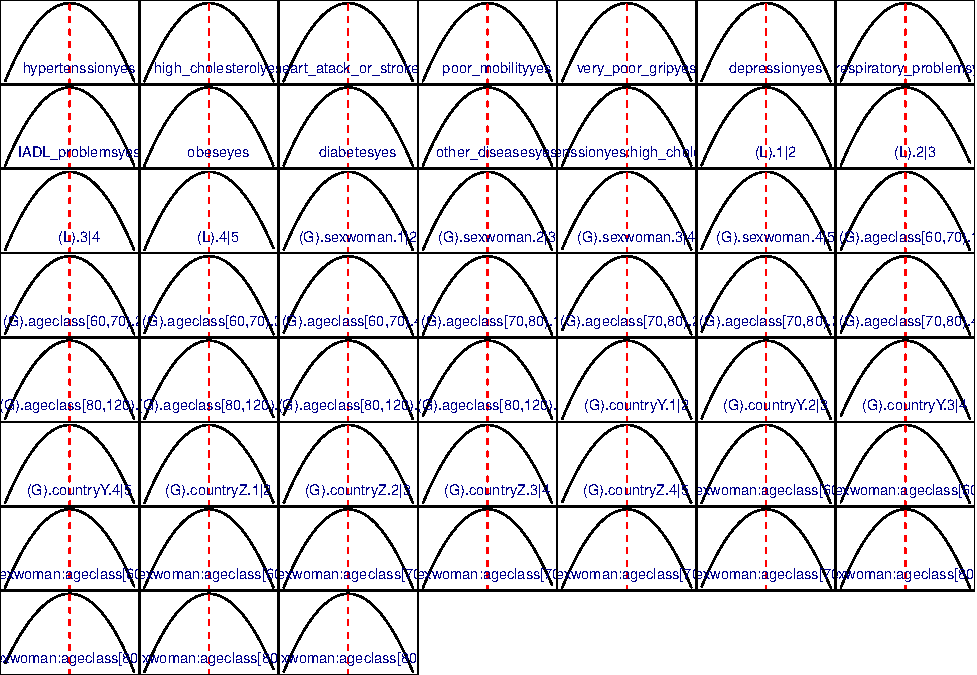
\includegraphics{vignette_files/figure-latex/unnamed-chunk-13-1.pdf}

\begin{verbatim}
## All parameters seem to be at arg.max (at optimum).
\end{verbatim}

\hypertarget{analyses-of-the-reporting-styles-using-hopit-package}{%
\subsection{\texorpdfstring{6. Analyses of the reporting styles using
\emph{hopit}
package}{6. Analyses of the reporting styles using hopit package}}\label{analyses-of-the-reporting-styles-using-hopit-package}}

Let's look at latent health variables of \emph{model2}.

\begin{Shaded}
\begin{Highlighting}[]
\NormalTok{model3}\OperatorTok{$}\NormalTok{coef.ls}\OperatorTok{$}\NormalTok{latent.params}
\end{Highlighting}
\end{Shaded}

\begin{verbatim}
##                     hypertenssionyes                  high_cholesterolyes 
##                           0.16692322                           0.04478911 
##             heart_atack_or_strokeyes                     poor_mobilityyes 
##                           0.35296700                           0.70450393 
##                    very_poor_gripyes                        depressionyes 
##                           0.51500758                           0.24905559 
##              respiratory_problemsyes                     IADL_problemsyes 
##                           0.37763441                           0.59062305 
##                             obeseyes                          diabetesyes 
##                           0.18939406                           0.33180729 
##                    other_diseasesyes hypertenssionyes:high_cholesterolyes 
##                           0.32861717                           0.08822596
\end{verbatim}

We can standardize them using Jürges' approach (Jürges 2007) to obtain
disability weights. The standardization can be doen using
\emph{standardizeCoef}() function.

\begin{Shaded}
\begin{Highlighting}[]
\CommentTok{# A function that modifies coefficient names.  }
\NormalTok{txtfun <-}\StringTok{ }\ControlFlowTok{function}\NormalTok{(x) }\KeywordTok{gsub}\NormalTok{(}\StringTok{'_'}\NormalTok{,}\StringTok{' '}\NormalTok{,}\KeywordTok{substr}\NormalTok{(x,}\DecValTok{1}\NormalTok{,}\KeywordTok{nchar}\NormalTok{(x)}\OperatorTok{-}\DecValTok{3}\NormalTok{))}

\CommentTok{# Calcualte and plot disability weights}
\NormalTok{sc <-}\StringTok{ }\KeywordTok{standardizeCoef}\NormalTok{(model3, }\DataTypeTok{plotf =} \OtherTok{TRUE}\NormalTok{, }\DataTypeTok{namesf =}\NormalTok{ txtfun)}
\end{Highlighting}
\end{Shaded}

\begin{center}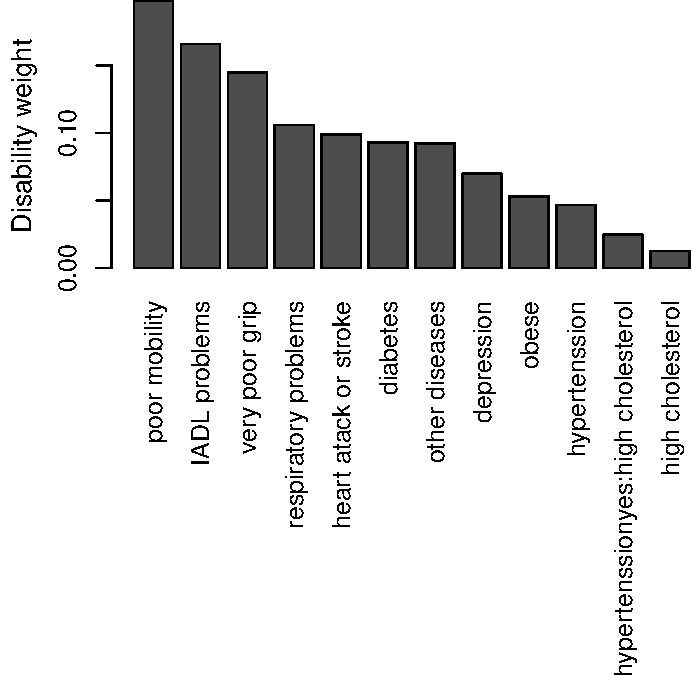
\includegraphics{vignette_files/figure-latex/unnamed-chunk-15-1} \end{center}

\begin{Shaded}
\begin{Highlighting}[]
\NormalTok{sc}
\end{Highlighting}
\end{Shaded}

\begin{verbatim}
##                                         [,1]
## poor mobility                     0.19778802
## IADL problems                     0.16581620
## very poor grip                    0.14458732
## respiratory problems              0.10602008
## heart atack or stroke             0.09909476
## diabetes                          0.09315421
## other diseases                    0.09225859
## depression                        0.06992184
## obese                             0.05317199
## hypertenssion                     0.04686335
## hypertenssionyes:high cholesterol 0.02476926
## high cholesterol                  0.01257445
\end{verbatim}

The \emph{namesf} argument is a function or a character vector that is
used to rename the coefficent names. Here, it removes last 3 letters
(``yes''), which is a reference level for each variable and exchanges
"\_" with spaces in variable names.

The latent index is simply calculated using \emph{latentindex}()
function.

\begin{Shaded}
\begin{Highlighting}[]
\NormalTok{hi <-}\StringTok{ }\KeywordTok{latentIndex}\NormalTok{(model3, }\DataTypeTok{plotf =} \OtherTok{TRUE}\NormalTok{, }\DataTypeTok{response =} \StringTok{"data"}\NormalTok{, }
                  \DataTypeTok{ylab =} \StringTok{'Health index'}\NormalTok{, }\DataTypeTok{col=}\StringTok{'deepskyblue3'}\NormalTok{)}
\end{Highlighting}
\end{Shaded}

\begin{center}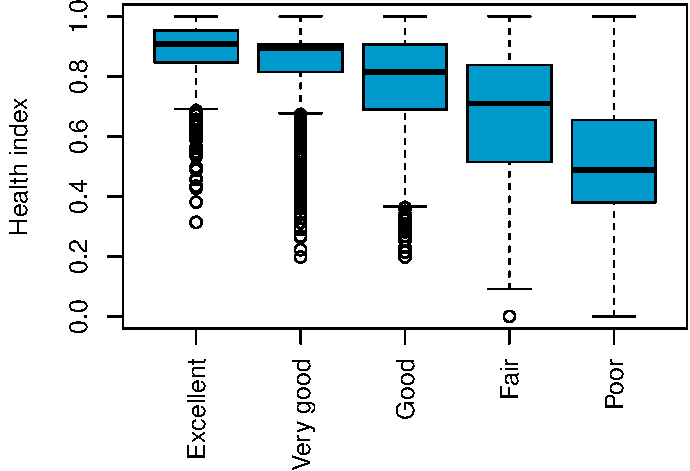
\includegraphics{vignette_files/figure-latex/unnamed-chunk-16-1} \end{center}

The boxplot shows reported health status vs.~health index. It is also
possible to plot expected categorical health status on Y axis calcualted
according to the eq. (2).

\begin{Shaded}
\begin{Highlighting}[]
\NormalTok{hi <-}\StringTok{ }\KeywordTok{latentIndex}\NormalTok{(model3, }\DataTypeTok{plotf =} \OtherTok{TRUE}\NormalTok{, }\DataTypeTok{response =} \StringTok{"fitted"}\NormalTok{, }
                  \DataTypeTok{ylab =} \StringTok{'Health index'}\NormalTok{, }\DataTypeTok{col=}\StringTok{'deepskyblue3'}\NormalTok{)}
\end{Highlighting}
\end{Shaded}

\begin{center}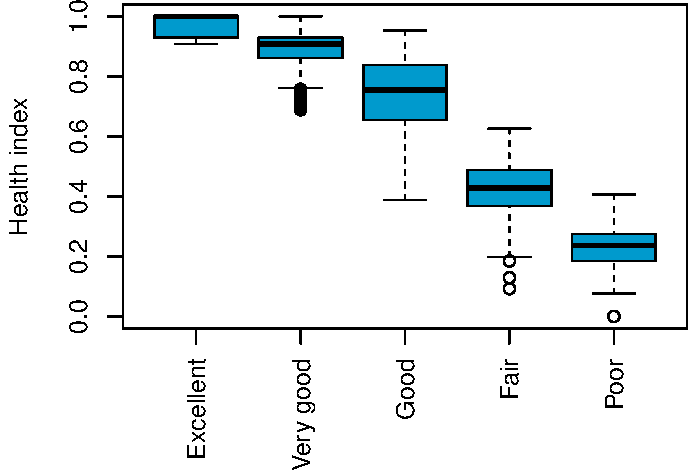
\includegraphics{vignette_files/figure-latex/unnamed-chunk-17-1} \end{center}

or according to Jürges' method:

\begin{Shaded}
\begin{Highlighting}[]
\NormalTok{hi <-}\StringTok{ }\KeywordTok{latentIndex}\NormalTok{(model3, }\DataTypeTok{plotf =} \OtherTok{TRUE}\NormalTok{, }\DataTypeTok{response =} \StringTok{"Jurges"}\NormalTok{, }
                  \DataTypeTok{ylab =} \StringTok{'Health index'}\NormalTok{, }\DataTypeTok{col=}\StringTok{'deepskyblue3'}\NormalTok{)}
\end{Highlighting}
\end{Shaded}

\begin{center}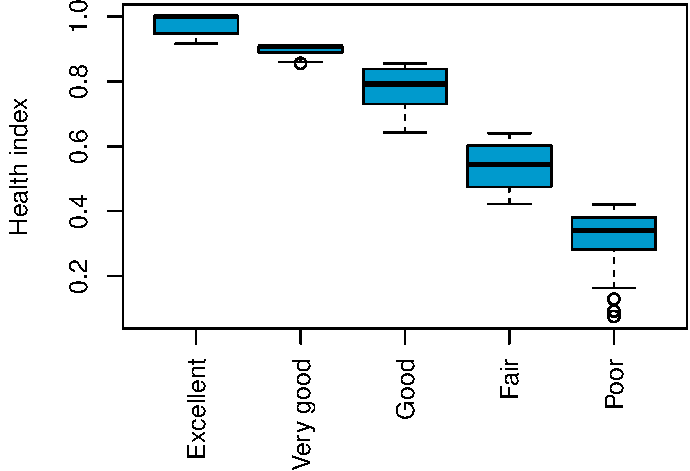
\includegraphics{vignette_files/figure-latex/unnamed-chunk-18-1} \end{center}

The central part of reporting styles analyses is to determine the
cut-points used to calcualte adjusted health status for each individual.
The calcualtion and ploting of cut-points is realized by
\emph{getCutPoints}() function.

\begin{Shaded}
\begin{Highlighting}[]
\NormalTok{z=}\KeywordTok{getCutPoints}\NormalTok{(}\DataTypeTok{model=}\NormalTok{model3)}
\end{Highlighting}
\end{Shaded}

\begin{center}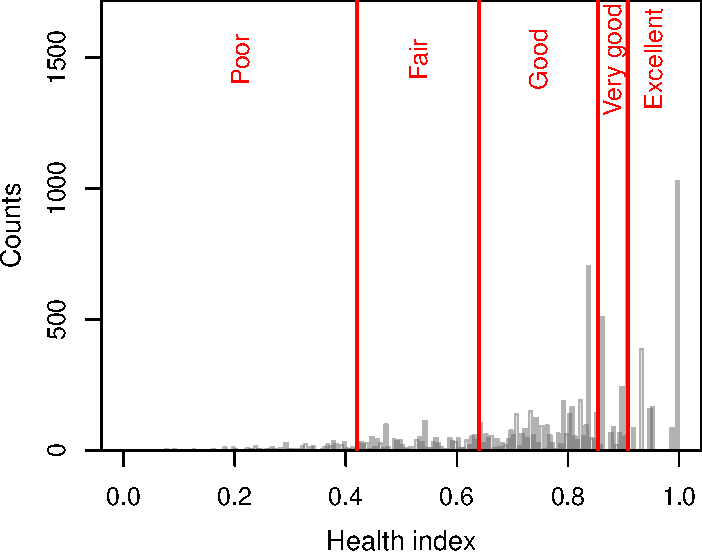
\includegraphics{vignette_files/figure-latex/unnamed-chunk-19-1} \end{center}

\begin{Shaded}
\begin{Highlighting}[]
\CommentTok{# Health index cut-points}
\NormalTok{z}\OperatorTok{$}\NormalTok{cutpoints}
\end{Highlighting}
\end{Shaded}

\begin{verbatim}
##     4.41%    17.68%    52.34%    77.63% 
## 0.4210433 0.6400315 0.8545694 0.9077414
\end{verbatim}

\begin{Shaded}
\begin{Highlighting}[]
\CommentTok{#Adjusted health levels for individuals: Jurges method}
\KeywordTok{table}\NormalTok{(z}\OperatorTok{$}\NormalTok{adjused.health.levels)}
\end{Highlighting}
\end{Shaded}

\begin{verbatim}
## 
##      Poor      Fair      Good Very good Excellent 
##       450      1347      3505      2787      1909
\end{verbatim}

\begin{Shaded}
\begin{Highlighting}[]
\CommentTok{#Adjusted health levels for individuals: Estimated model thresholds}
\KeywordTok{table}\NormalTok{(model3}\OperatorTok{$}\NormalTok{Ey_i)}
\end{Highlighting}
\end{Shaded}

\begin{verbatim}
## 
## Excellent Very good      Good      Fair      Poor 
##       737      4361      4029       807        66
\end{verbatim}

\begin{Shaded}
\begin{Highlighting}[]
\CommentTok{#Original health levels for individuals}
\KeywordTok{table}\NormalTok{(model3}\OperatorTok{$}\NormalTok{y_i)}
\end{Highlighting}
\end{Shaded}

\begin{verbatim}
## 
## Excellent Very good      Good      Fair      Poor 
##      2237      2529      3466      1327       441
\end{verbatim}

The analysis of health levels is done by \emph{getLevels}() function

\begin{Shaded}
\begin{Highlighting}[]
\CommentTok{# Health levels for combination of age and gender, and pooled country of origin.}
\NormalTok{hl <-}\StringTok{ }\KeywordTok{getLevels}\NormalTok{(}\DataTypeTok{model=}\NormalTok{model3, }\DataTypeTok{formula=}\OperatorTok{~}\StringTok{ }\NormalTok{sex }\OperatorTok{+}\StringTok{ }\NormalTok{ageclass, }\DataTypeTok{data =}\NormalTok{ healthsurvey, }
                      \DataTypeTok{sep=}\StringTok{' '}\NormalTok{, }\DataTypeTok{plotf=}\OtherTok{TRUE}\NormalTok{, }\DataTypeTok{legbty =} \StringTok{'n'}\NormalTok{)}
\end{Highlighting}
\end{Shaded}

\begin{center}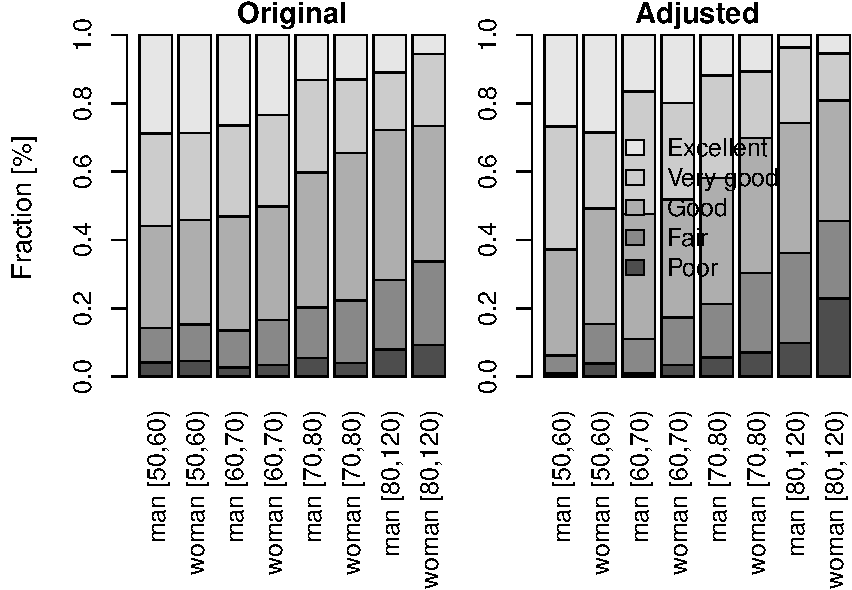
\includegraphics{vignette_files/figure-latex/unnamed-chunk-20-1} \end{center}

The differences between original and adjusted frequncies can be
calcualted directly using \emph{getLevels} output:

\begin{Shaded}
\begin{Highlighting}[]
\KeywordTok{round}\NormalTok{(}\DecValTok{100}\OperatorTok{*}\NormalTok{(hl}\OperatorTok{$}\NormalTok{original }\OperatorTok{-}\StringTok{ }\NormalTok{hl}\OperatorTok{$}\NormalTok{adjusted),}\DecValTok{2}\NormalTok{)}
\end{Highlighting}
\end{Shaded}

\begin{verbatim}
##                 
##                    Poor   Fair   Good Very good Excellent
##   man [50,60)      3.28   4.77  -1.15     -9.02      2.13
##   woman [50,60)    0.77  -1.03  -3.09      3.13      0.21
##   man [60,70)      1.66   0.77  -3.19     -9.26     10.03
##   woman [60,70)    0.06  -0.87  -1.25     -1.50      3.55
##   man [70,80)     -0.19  -0.86   2.68     -3.07      1.44
##   woman [70,80)   -3.09  -4.97   3.75      1.97      2.34
##   man [80,120)    -1.87  -6.07   5.84     -5.14      7.24
##   woman [80,120) -13.55   1.64   4.31      7.39      0.21
\end{verbatim}

\hypertarget{bootstraping-confidence-intervals}{%
\subsection{7. Bootstraping Confidence
Intervals}\label{bootstraping-confidence-intervals}}

The package offers functions to calculate confidence intervals for any
measure derived from the model. As an example we show calcualtion of
confidence intervals of the difference between original and adjusted
frequencies of combined ``Poor'' + ``Fair'' healt categories.

\begin{Shaded}
\begin{Highlighting}[]
\CommentTok{# Function to be bootstraped}
\NormalTok{diff_BadHealth <-}\StringTok{ }\ControlFlowTok{function}\NormalTok{(model, data) \{}
\NormalTok{  hl <-}\StringTok{ }\KeywordTok{getLevels}\NormalTok{(}\DataTypeTok{model=}\NormalTok{model, }\DataTypeTok{formula=}\OperatorTok{~}\StringTok{ }\NormalTok{sex }\OperatorTok{+}\StringTok{ }\NormalTok{ageclass, }\DataTypeTok{data =}\NormalTok{ data, }
                  \DataTypeTok{sep=}\StringTok{' '}\NormalTok{, }\DataTypeTok{plotf=}\OtherTok{FALSE}\NormalTok{)}
\NormalTok{  hl}\OperatorTok{$}\NormalTok{original[,}\DecValTok{1}\NormalTok{] }\OperatorTok{+}\StringTok{ }\NormalTok{hl}\OperatorTok{$}\NormalTok{original[,}\DecValTok{2}\NormalTok{] }\OperatorTok{-}\StringTok{ }\NormalTok{hl}\OperatorTok{$}\NormalTok{adjusted[,}\DecValTok{1}\NormalTok{]}\OperatorTok{-}\StringTok{ }\NormalTok{hl}\OperatorTok{$}\NormalTok{adjusted[,}\DecValTok{2}\NormalTok{]}
\NormalTok{\}}

\CommentTok{# Estimate of the difference}
\NormalTok{est.org <-}\StringTok{ }\KeywordTok{diff_BadHealth}\NormalTok{(}\DataTypeTok{model =}\NormalTok{ model3, }\DataTypeTok{data =}\NormalTok{ healthsurvey)}

\CommentTok{# Perform the bootstrap}
\NormalTok{B <-}\StringTok{ }\KeywordTok{boot_hopit}\NormalTok{(}\DataTypeTok{model =}\NormalTok{ model3, }\DataTypeTok{data =}\NormalTok{ healthsurvey, }
                \DataTypeTok{func =}\NormalTok{ diff_BadHealth, }\DataTypeTok{nboot =} \DecValTok{100}\NormalTok{)}

\CommentTok{# Calcualte lower and upper bounds using percentile method}
\NormalTok{est.CI <-}\StringTok{ }\KeywordTok{boot_hopit_CI}\NormalTok{(B)}

\CommentTok{# Plotting the difference and its (assymetrical) confidence intervals}
\NormalTok{pmar <-}\StringTok{ }\KeywordTok{par}\NormalTok{(}\StringTok{'mar'}\NormalTok{); }\KeywordTok{par}\NormalTok{(}\DataTypeTok{mar =} \KeywordTok{c}\NormalTok{(}\FloatTok{9.5}\NormalTok{,pmar[}\DecValTok{2}\OperatorTok{:}\DecValTok{4}\NormalTok{]))}
\NormalTok{m <-}\StringTok{ }\KeywordTok{max}\NormalTok{(}\KeywordTok{abs}\NormalTok{(est.CI))}
\NormalTok{pos <-}\StringTok{ }\KeywordTok{barplot}\NormalTok{(est.org, }\DataTypeTok{names.arg =} \KeywordTok{names}\NormalTok{(est.org), }\DataTypeTok{las =} \DecValTok{3}\NormalTok{, }\DataTypeTok{ylab =} \StringTok{'Orginal - Adjusted'}\NormalTok{, }
               \DataTypeTok{ylim=}\KeywordTok{c}\NormalTok{(}\OperatorTok{-}\NormalTok{m, m), }\DataTypeTok{density =} \DecValTok{20}\NormalTok{, }\DataTypeTok{angle =} \KeywordTok{c}\NormalTok{(}\DecValTok{45}\NormalTok{, }\DecValTok{-45}\NormalTok{), }\DataTypeTok{col =} \KeywordTok{c}\NormalTok{(}\StringTok{'blue'}\NormalTok{, }\StringTok{'orange'}\NormalTok{))}
\ControlFlowTok{for}\NormalTok{ (k }\ControlFlowTok{in} \KeywordTok{seq_along}\NormalTok{(pos)) }\KeywordTok{lines}\NormalTok{(}\KeywordTok{c}\NormalTok{(pos[k,}\DecValTok{1}\NormalTok{],pos[k,}\DecValTok{1}\NormalTok{]), est.CI[,k], }\DataTypeTok{lwd =} \DecValTok{2}\NormalTok{, }\DataTypeTok{col =} \DecValTok{2}\NormalTok{)}
\KeywordTok{abline}\NormalTok{(}\DataTypeTok{h =} \DecValTok{0}\NormalTok{); }\KeywordTok{box}\NormalTok{(); }\KeywordTok{par}\NormalTok{(}\DataTypeTok{mar =}\NormalTok{ pmar)}
\end{Highlighting}
\end{Shaded}

\begin{center}\includegraphics{vignette_files/figure-latex/unnamed-chunk-22-1} \end{center}

The results show that men tend to over-report bad health at ages
(50,60{]} and (50,70{]}, wherease women at ages {[}70,80) and both sexes
at ages (80, 120{]} under-report bad health.

\hypertarget{references}{%
\subsection*{8. References}\label{references}}
\addcontentsline{toc}{subsection}{8. References}

\hypertarget{refs}{}
\leavevmode\hypertarget{ref-Boes2006}{}%
Boes, Stefan, and Rainer Winkelmann. 2006. ``Ordered Response Models.''
\emph{Allgemeines Statistisches Archiv} 90 (1): 167--81.
\url{https://doi.org/10.1007/s10182-006-0228-y}.

\leavevmode\hypertarget{ref-Green2014}{}%
Greene, William, Mark N. Harris, Bruce Hollingsworth, and Timothy A.
Weterings. 2014. ``Heterogeneity in Ordered Choice Models: A Review with
Applications to Self-Assessed Health.'' \emph{Journal of Economic
Surveys} 28 (1): 109--33. \url{https://doi.org/10.1111/joes.12002}.

\leavevmode\hypertarget{ref-GreeneHensher2010}{}%
Greene, William, and David Hensher. 2010. \emph{Modeling Ordered
Choices}. Cambridge University Press.
\url{https://EconPapers.repec.org/RePEc:cup:cbooks:9780521142373}.

\leavevmode\hypertarget{ref-Terza1985}{}%
Ierza, Joseph V. 1985. ``Ordinal Probit: A Generalization.''
\emph{Communications in Statistics - Theory and Methods} 14 (1). Taylor
\& Francis: 1--11. \url{https://doi.org/10.1080/03610928508828893}.

\leavevmode\hypertarget{ref-Jurges2007}{}%
Jürges, Hendrik. 2007. ``True Health Vs Response Styles: Exploring
Cross-Country Differences in Self-Reported Health.'' \emph{Health
Economics} 16 (2): 163--78. \url{https://doi.org/10.1002/hec.1134}.

\leavevmode\hypertarget{ref-King2004}{}%
King, Gary, Christopher J. L. Murray, Joshua A. Salomon, and Ajay
Tandon. 2004. ``Enhancing the Validity and Cross-Cultural Comparability
of Measurement in Survey Research.'' \emph{American Political Science
Review} 98 (1). Cambridge University Press: 191--207.
\url{https://doi.org/10.1017/S000305540400108X}.

\leavevmode\hypertarget{ref-Liao2005}{}%
Liao, Pei-Shan, Yang-Chih Fu, and Chin-Chun Yi. 2005. ``Perceived
Quality of Life in Taiwan and Hong Kong: An Intra-Culture Comparison.''
\emph{Journal of Happiness Studies} 6 (1): 43--67.
\url{https://doi.org/10.1007/s10902-004-1753-6}.

\leavevmode\hypertarget{ref-McKelvey1975}{}%
McKelvey, R. D., and W. Zavoina. 1975. ``A Statistical Model for the
Analysis of Ordinal Level Dependent Variables.'' \emph{Journal of
Mathematical Sociology} 4 (1): 103--20.

\leavevmode\hypertarget{ref-Rebelo2014}{}%
Rebelo, Luis Pina, and Nuno Sousa Pereira. 2014. ``Assessing Health
Endowment, Access and Choice Determinants: Impact on Retired Europeans'
(in)activity and Quality of Life.'' \emph{Social Indicators Research}
119 (3). Germany: Springer: 1411--46.
\url{https://doi.org/10.1007/s11205-013-0542-1}.


\end{document}
